%
%
\subsection{Definition}
%
In this example the aquifer consists of a small strip with the size of 100~m $\times$ 2~m (see Fig.~\ref{GW_Results_uc}). At both ends the head is fixed and constant recharge is imposed on the whole domain which leads to steady state flow. This setting allows the comparison with an analytical solution.
%\emph{uc\_quad}, \emph{uc\_tri} solve the two-dimensional Eqn.~\ref{eqn:GW_unconfinedGoverning}  for unconfined auifer and \emph{uc\_pris} solves the three-dimensional groundwater Eqn.\ref{eqn:GW_Governing}.
%
Initial groundwater head is 0 m. At one end of the strip the head is 1~m at the other 5~m. At the top a source term is 1.0$\times 10^{-8}$ m/s and at the remaining parts no-flow is imposed.
%
For the spatial discretization 100 equal quadrants and 410 triangles or prisms are used. In the later case, the three-dimensional unconfined groundwater equation is solved with elements adapting to the water height. One time step with the size of 100~s is used. The specific storage $S_s = 0$ m $^{-1}$ or specific yield $S_y = 0$ and a hydraulic conductivity $K$ of 9.9$\times 10^{-6}$ m/s are used.

\subsection{Analytical solution}
In an unconfined aquifer, the saturated thickness is defined as the vertical distance between the water table surface and the aquifer base. If the aquifer base is at the zero datum, then the unconfined saturated thickness ($b$) is equal to the head ($h$).
With the Dupuit assumption (or Dupuit-Forcheimer assumption), where it is assumed that heads do not vary in the vertical direction (i.e., $ \frac {\partial h} {\partial z}=0$), a horizontal water balance is only applied to a long vertical column with area ($\delta x \delta y$) extending from the aquifer base to the unsaturated surface. For this vertical column, applying Dacy's law and mass balance expression, the groundwater flow equation for unconfined aquifer can be obtained:

\begin{eqnarray}
S_y \frac {\partial h} {\partial t} = \nabla\cdot(kh\nabla h) +N
\label{GW_unconfinedEq1}
\end{eqnarray}

where N is the source term [L/T], represents the addition of water in the vertical direction, $S_y$ is the specific yield of the aquifer [-], $k$ is the hydraulic conductivity [L/T].

The unconfined groundwater flow equation is non-linear partial differential equation, for steady-state flow,  it may be linearized by expressing the PDE in terms of the squared head:

\begin{eqnarray}
 \nabla\cdot(k\nabla h^2) = -2N
\label{GW_unconfinedEq2}
\end{eqnarray}

and for the homogeneous aquifers, Eq.~\ref{GW_unconfinedEq2} becomes

\begin{eqnarray}
 \nabla ^2 \nabla h^2 = - \frac{2N}{k}
\label{GW_unconfinedEq3}
\end{eqnarray}

Eq.~\ref{GW_unconfinedEq3} can be solved by the standard integration method for linear PDEs. For the definition of the unconfined aquifer above, the analytical solution is expressed by the following equation.

\begin{eqnarray}
 h=\sqrt{-0.001 x^2-0.14x+25}
\label{UGW_analytical}
\end{eqnarray}  
%
\subsection{Results}
%
Comparison of simulation results with prisms and analytical solution is shown in Fig.~\ref{GW_Results_uc}.
%
\begin{figure} [H]
 \centering
 \vspace{-10pt}
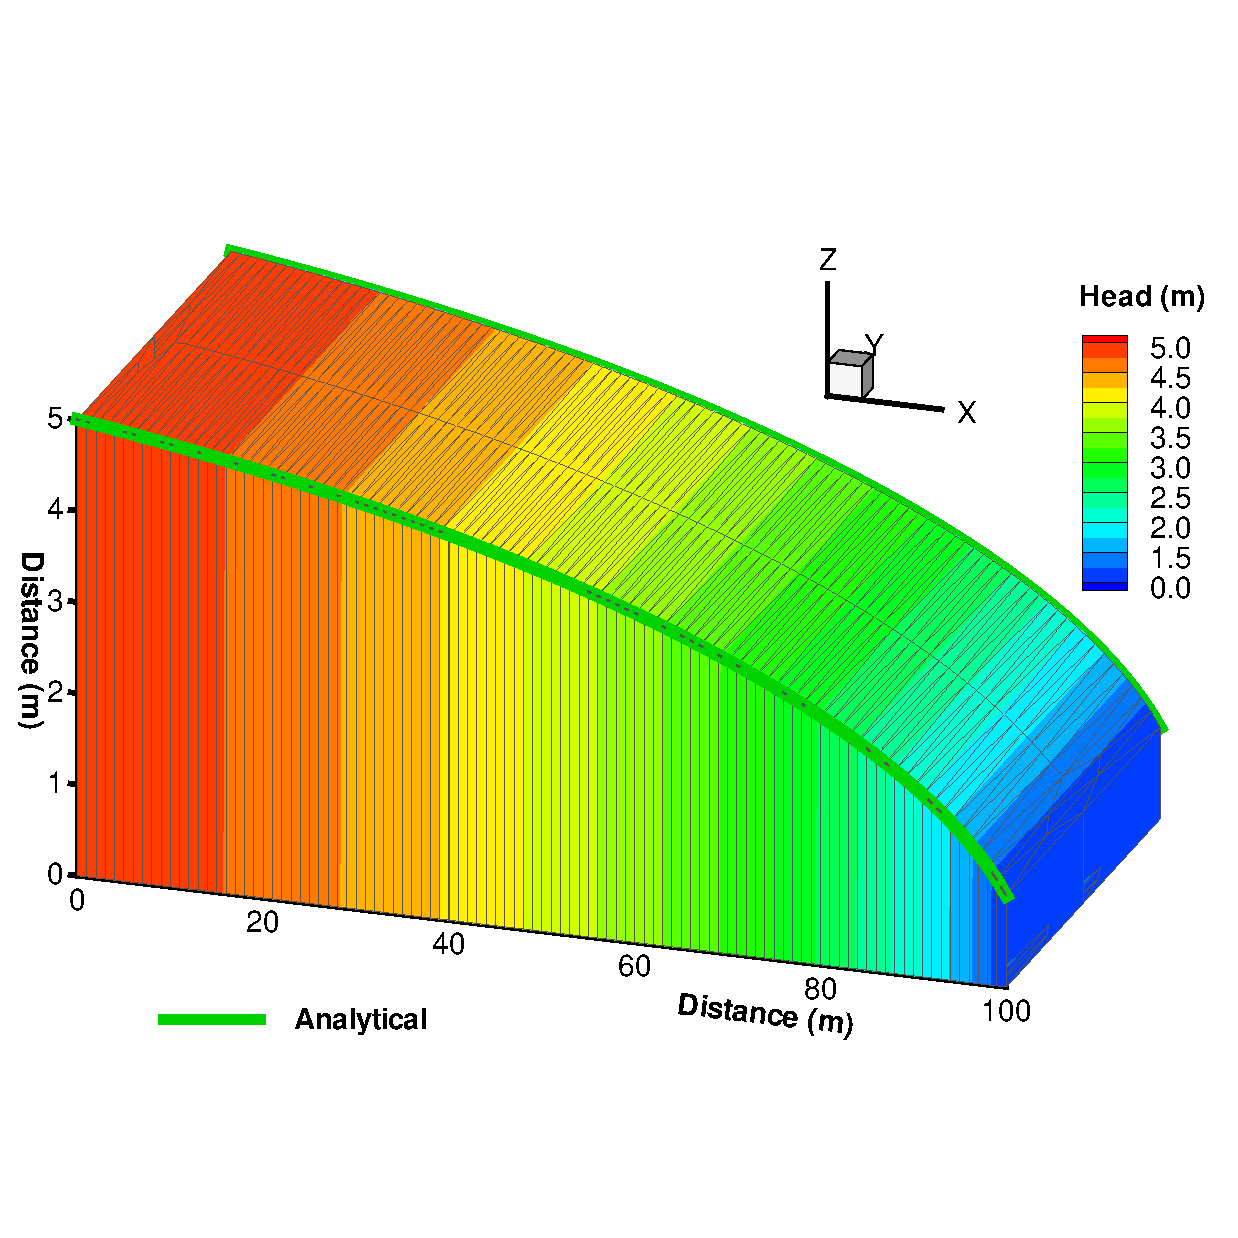
\includegraphics[width=0.7\columnwidth] {Chapter5/figure/uc_pris.eps}
\vspace{-10pt}
\caption{Benchmark example results of unconfined aquifer with prisms.}
\vspace{-10pt}
 \label{GW_Results_uc}
\end{figure}
%
